\section{SoCPilot Framework}
Application-driven SoC customization requires coordinated decisions across application analysis, hardware/software partitioning, accelerator implementation, and system integration. These decisions are coupled: accelerating a compute-intensive function may provide little application-level benefit once communication overhead and hardware cost are considered. To coordinate these decisions with quantitative tool feedback, we develop SoCPilot, an agentic framework that transforms application requirements and C/C++ code into a customized CPU--accelerator SoC and supports its optimization and FPGA validation.

\subsection{SoCPilot Overview}
\label{sec:socpilot-overview}
Figure~\ref{fig: overview} presents the overall architecture of SoCPilot. The framework combines LLM-based orchestration, reusable case and IP libraries, and a toolchain for profiling, hardware generation, simulation, and synthesis. The LLM interprets requirements and coordinates the design stages, while the libraries supply reusable system components and the tools provide implementation artifacts, correctness checks, and quantitative cost estimates.

The design flow consists of four stages. First, requirement interpretation and IP selection convert user requirements into a structured specification and an initial manifest of reusable system IPs. Second, application profiling and hardware/software partitioning identify candidate functions, evaluate their hardware implementations, and select an accelerator set using latency, communication, and area estimates. Third, SoC generation and design space exploration (DSE) package and integrate the selected accelerators and refine processor, memory-system, and accelerator configurations under latency and area objectives. Finally, FPGA prototyping and board validation invoke the ESP implementation flow to generate a bitstream and validate the resulting system. Structured specifications, task graphs, and SoC configurations connect these stages, with tool feedback guiding design refinement. The following subsections describe the four components in detail.

\subsection{Requirement Interpretation and IP Selection}
The first stage determines the reusable system components required by the target application. Directly mapping natural-language descriptions to concrete IP instances is unreliable because user terminology, IP metadata, and hardware interfaces are expressed at different abstraction levels. SoCPilot therefore separates requirement interpretation from IP retrieval. As shown in Figure \ref{fig:soc-spec}, the LLM first converts the user description into a structured SoC specification and then uses this specification to query a hierarchical library of verified IPs.

\begin{figure*}[htp]
    \centering
    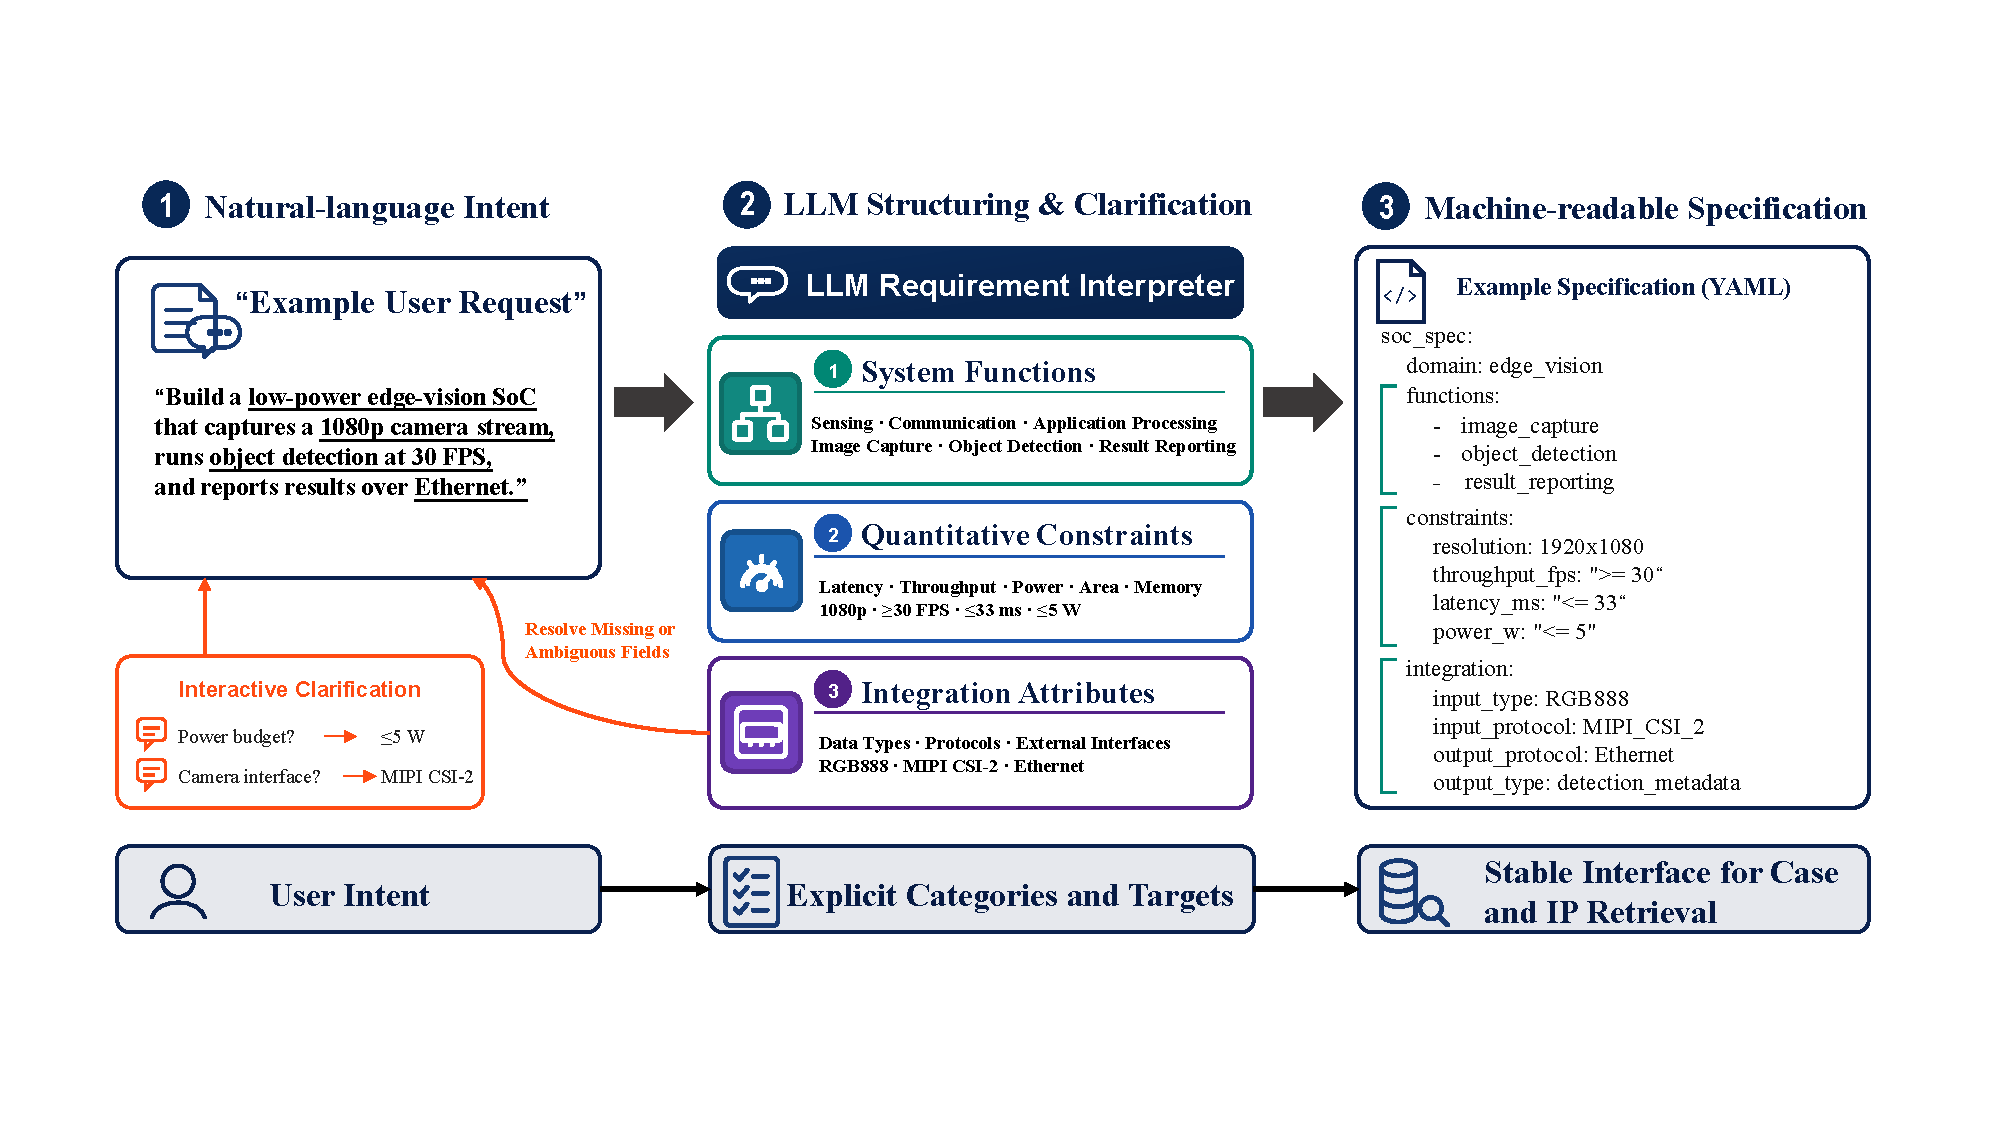
\includegraphics[width=0.95\textwidth,trim=0bp 84bp 0bp 78bp,clip]{pic/soc-spec.pdf} 
    \caption{Structured SoC specification generation. The LLM translates natural-language requirements into system functions, quantitative constraints, and integration attributes, while resolving missing or ambiguous fields through interactive clarification. The example illustrates the resulting machine-readable specification used for subsequent case and IP retrieval.}
\label{fig:soc-spec}
    \vspace{-1em}
\end{figure*}



The structured specification records three types of information: (1) the required system functions, such as sensing, communication, and application processing; (2) quantitative constraints, including latency, throughput, power, area, and memory capacity; and (3) integration attributes, such as data types, protocols, and external interfaces. Missing or ambiguous fields trigger an interactive clarification step. This representation decomposes a high-level application scenario into explicit IP categories and target specifications, providing a stable interface between user intent and the implementation flow.

\begin{table*}[htb]
\centering
\begin{threeparttable}
  \caption{Requirement-to-IP Taxonomy for SoC Customization}
  \label{tab:req_taxonomy}
  \begin{tabularx}{0.8\linewidth}{cllX}
    \toprule
    \textbf{Tier\tnote{a}} & \textbf{Category} & \textbf{Tag} & \textbf{Description / Examples} \\
    \midrule
    \multirow{1}{*}{T0} 
      & Application Domain       & \texttt{domain} & AI inference, sensor hub, audio DSP, ISPs, etc. \\
    \midrule
    \multirow{4}{*}{T1}
      & Compute                  & \texttt{cpu}, \texttt{dsp}, \texttt{ai} & RISC-V, Arm cores, DSPs, AI accelerators\\
      & Memory and Cache         & \texttt{mem}     & DDR/LPDDR, SRAM, cache hierarchy and coherency, scratchpad \\
      & Interconnect             & \texttt{noc}, \texttt{axi}, \texttt{pcie} & Mesh NoC, AXI buses, PCIe root complex \\
      & I/O Interfaces           & \texttt{io}      & USB, SPI, I2C, CAN, MIPI CSI/DSI, GPIO \\
    \midrule
    \multirow{4}{*}{T2}
      & Power and Energy         & \texttt{power}   & Power budget, DVFS, retention memory \\
      & Security and Safety      & \texttt{sec}     & AES engine, secure boot, ASIL level \\
      & Reliability / Lifetime   & \texttt{rel}     & ECC, watchdog, over-temperature protection \\
      & Thermal and Packaging    & \texttt{pkg}     & Thermal budget, packaging constraints \\
    \midrule
    \multirow{1}{*}{T3}
      & Integration Constraints  & \texttt{pkg}     & I/O count, physical interface compatibility (e.g., PHYs, pads) \\
    \bottomrule
  \end{tabularx}
  
  % 表格下方的注释区域
  \begin{tablenotes}
    \footnotesize
    \item[a] T0 identifies the application domain; T1 describes primary hardware components; T2 captures cross-layer constraints; and T3 records implementation and integration constraints.
  \end{tablenotes}
  
\end{threeparttable}
\end{table*}

Table~\ref{tab:req_taxonomy} summarizes the taxonomy used to organize both requirements and IP metadata. Each library entry contains a functional description, supported configurations, interface protocols, resource and performance characterization, verification status, and known dependencies. SoCPilot first retrieves semantically similar verified designs from a case library. If no case provides a compatible configuration, the LLM decomposes the structured specification into IP queries, retrieves candidates from the hierarchical IP library, and filters them using hard constraints such as protocol compatibility, capacity, and resource limits. The remaining candidates are ranked by their match to the requested performance targets.

The output of this stage is a machine-readable SoC manifest that records the selected processor, memory hierarchy, interconnect, I/O components, and their initial configurations. Application-specific compute kernels are not assumed to exist in the reusable IP library; instead, their accelerator implementations are determined by the profiling and hardware/software partitioning stage described next. This separation prevents the requirement interpreter from prematurely deciding which application functions should be implemented in hardware.

\subsection{Application Profiling and Hardware/Software Partitioning}
The second stage determines which application functions should remain on the CPU and which should be implemented as custom accelerators. Hotspot detection alone cannot make this decision: a frequently executed function may provide little net benefit after accelerator latency, hardware cost, invocation overhead, and data movement are considered. SoCPilot therefore treats profiling as candidate extraction and defers the mapping decision to an explicit hardware/software partitioning model.

\textbf{Application profiling and candidate extraction.}
SoCPilot compiles and executes the application with representative inputs and uses Callgrind to collect function-level instruction counts, call frequencies, and calling relationships. System routines, library wrappers, initialization code, and error-handling paths are removed from the profile, leaving application-defined functions that account for substantial execution time. A lightweight static pass then extracts each candidate with its type definitions and calling context and records potential synthesis obstacles, including recursion, dynamic allocation, irregular pointer accesses, and complex control flow. This pass determines whether a function can be evaluated by the HLS flow; it does not decide whether the function should be mapped to hardware. The LLM combines the dynamic profile and static call information into a task graph $G=(V,E)$, where nodes represent profiled functions and edges record control and data dependencies.

\textbf{LLM-assisted hardware evaluation.}
For each candidate hotspot, SoCPilot reuses the LLM-guided HLS generation and optimization procedure introduced in HLSPilot \cite{xiong2024hlspilot}. The LLM isolates or refactors the candidate into synthesizable C/C++, generates a functional testbench, and iteratively inserts HLS pragmas for pipelining, loop unrolling, and array partitioning. HLS reports provide the latency of one accelerator invocation and the synthesis information used by the common analytical area model to obtain an accelerator-area estimate $a_i$. The per-invocation latency is multiplied by the profiled call count to obtain the workload-level accelerator time $t_i^{\mathrm{acc}}$. Candidates that fail synthesis or verification remain software tasks; candidates with valid implementations proceed to the partitioning algorithm, even when their estimated area is high. Thus, HLS compatibility, latency, and area cost are measured or tool-derived rather than inferred from source appearance alone.

\textbf{CPU and communication models.}
The workload-level CPU latency $t_i^{\mathrm{cpu}}$ of each task is obtained from profiling and fast simulation with Sniper \cite{sniper}. For a hardware task, the model also accumulates accelerator launch and synchronization overhead as $t_i^{\mathrm{launch}}$. Each dependency $(i,j)\in E$ is annotated with its aggregate transfer volume $D_{ij}$ over the representative execution. If two dependent tasks are placed in different execution domains, their communication cost is approximated as
\begin{equation}
c_{ij}(x_i,x_j)=
\mathbb{I}[x_i\neq x_j]\left(L_{\mathrm{if}}+\frac{D_{ij}}{B_{\mathrm{if}}}\right),
\end{equation}
where $x_i\in\{0,1\}$ denotes software or hardware execution, and $L_{\mathrm{if}}$ and $B_{\mathrm{if}}$ are the interface latency and effective bandwidth. The execution cost of task $i$ is
\begin{equation}
d_i(x_i)=(1-x_i)t_i^{\mathrm{cpu}}+
x_i\left(t_i^{\mathrm{acc}}+t_i^{\mathrm{launch}}\right).
\end{equation}

\textbf{Partitioning formulation and algorithm.}
Given these estimates, SoCPilot minimizes the predicted completion time of the task graph subject to the application-specific area budget:
\begin{equation}
\begin{aligned}
\min_{\mathbf{x}}\quad &T_{\mathrm{app}}(\mathbf{x})
=\operatorname{Makespan}\!\left(G,\{d_i\},\{c_{ij}\}\right),\\
\mathrm{s.t.}\quad &\sum_{i\in V}x_i a_i\leq A^{\max}.
\end{aligned}
\label{eq:partition}
\end{equation}
Non-candidate functions are fixed to software. The implementation uses the marginal-gain heuristic in Algorithm~\ref{alg:hw-sw-partitioning}. Starting from an all-software mapping, it tentatively maps each feasible candidate to hardware, recomputes the task-graph completion time including boundary communication, and selects the candidate with the largest latency reduction per normalized unit of estimated area. The process stops when no feasible candidate produces a positive end-to-end benefit.

\begin{algorithm}
\caption{Hardware/Software Partitioning}
\label{alg:hw-sw-partitioning}
\KwIn{Task graph $G=(V,E)$; candidates $C$; timing estimates; area estimates $a_i$; area budget $A^{\max}$}
\KwOut{Hardware set $T_H$ and software set $T_S$}

$x_i\leftarrow 0,\ \forall i\in V$; $A_{\mathrm{used}}\leftarrow 0$\;
\While{true}{
    $C_f\leftarrow\{i\in C\mid x_i=0,\ A_{\mathrm{used}}+a_i\leq A^{\max}\}$\;
    \If{$C_f=\emptyset$}{break\;}
    \ForEach{$i\in C_f$}{
        $\mathbf{x}^{(i)}\leftarrow\mathbf{x}$; $x_i^{(i)}\leftarrow 1$\;
        $\Delta_i\leftarrow T_{\mathrm{app}}(\mathbf{x})
        -T_{\mathrm{app}}(\mathbf{x}^{(i)})$\;
        $\rho_i\leftarrow a_i/A^{\max}$\;
        $s_i\leftarrow\Delta_i/\rho_i$\;
    }
    $i^\star\leftarrow\arg\max_{i\in C_f}s_i$\;
    \If{$\Delta_{i^\star}\leq 0$}{break\;}
    $x_{i^\star}\leftarrow 1$\;
    $A_{\mathrm{used}}\leftarrow A_{\mathrm{used}}+a_{i^\star}$\;
}
$T_H\leftarrow\{i\mid x_i=1\}$\;
$T_S\leftarrow V\setminus T_H$\;
\Return{$T_H,T_S$}
\end{algorithm}

The resulting partition fixes the accelerator set and provides the initial architecture for SoC generation. The subsequent DSE stage fine-tunes processor, memory-system, interconnect, and accelerator parameters without repeatedly changing this mapping. Only when no feasible design can be found under the specified constraints does SoCPilot return to the partitioning stage and revise the hardware task set.

\subsection{SoC Generation and Design Space Exploration}\label{sec:soc-generation}
As shown in Figure \ref{fig:soc-generation}, the third stage transforms the IP manifest and hardware/software partition into an executable SoC. The partition determines the coarse CPU--accelerator organization, and DSE subsequently refines the parameters of that organization using more accurate system-level feedback.

\begin{figure*}[htp]
    \centering
    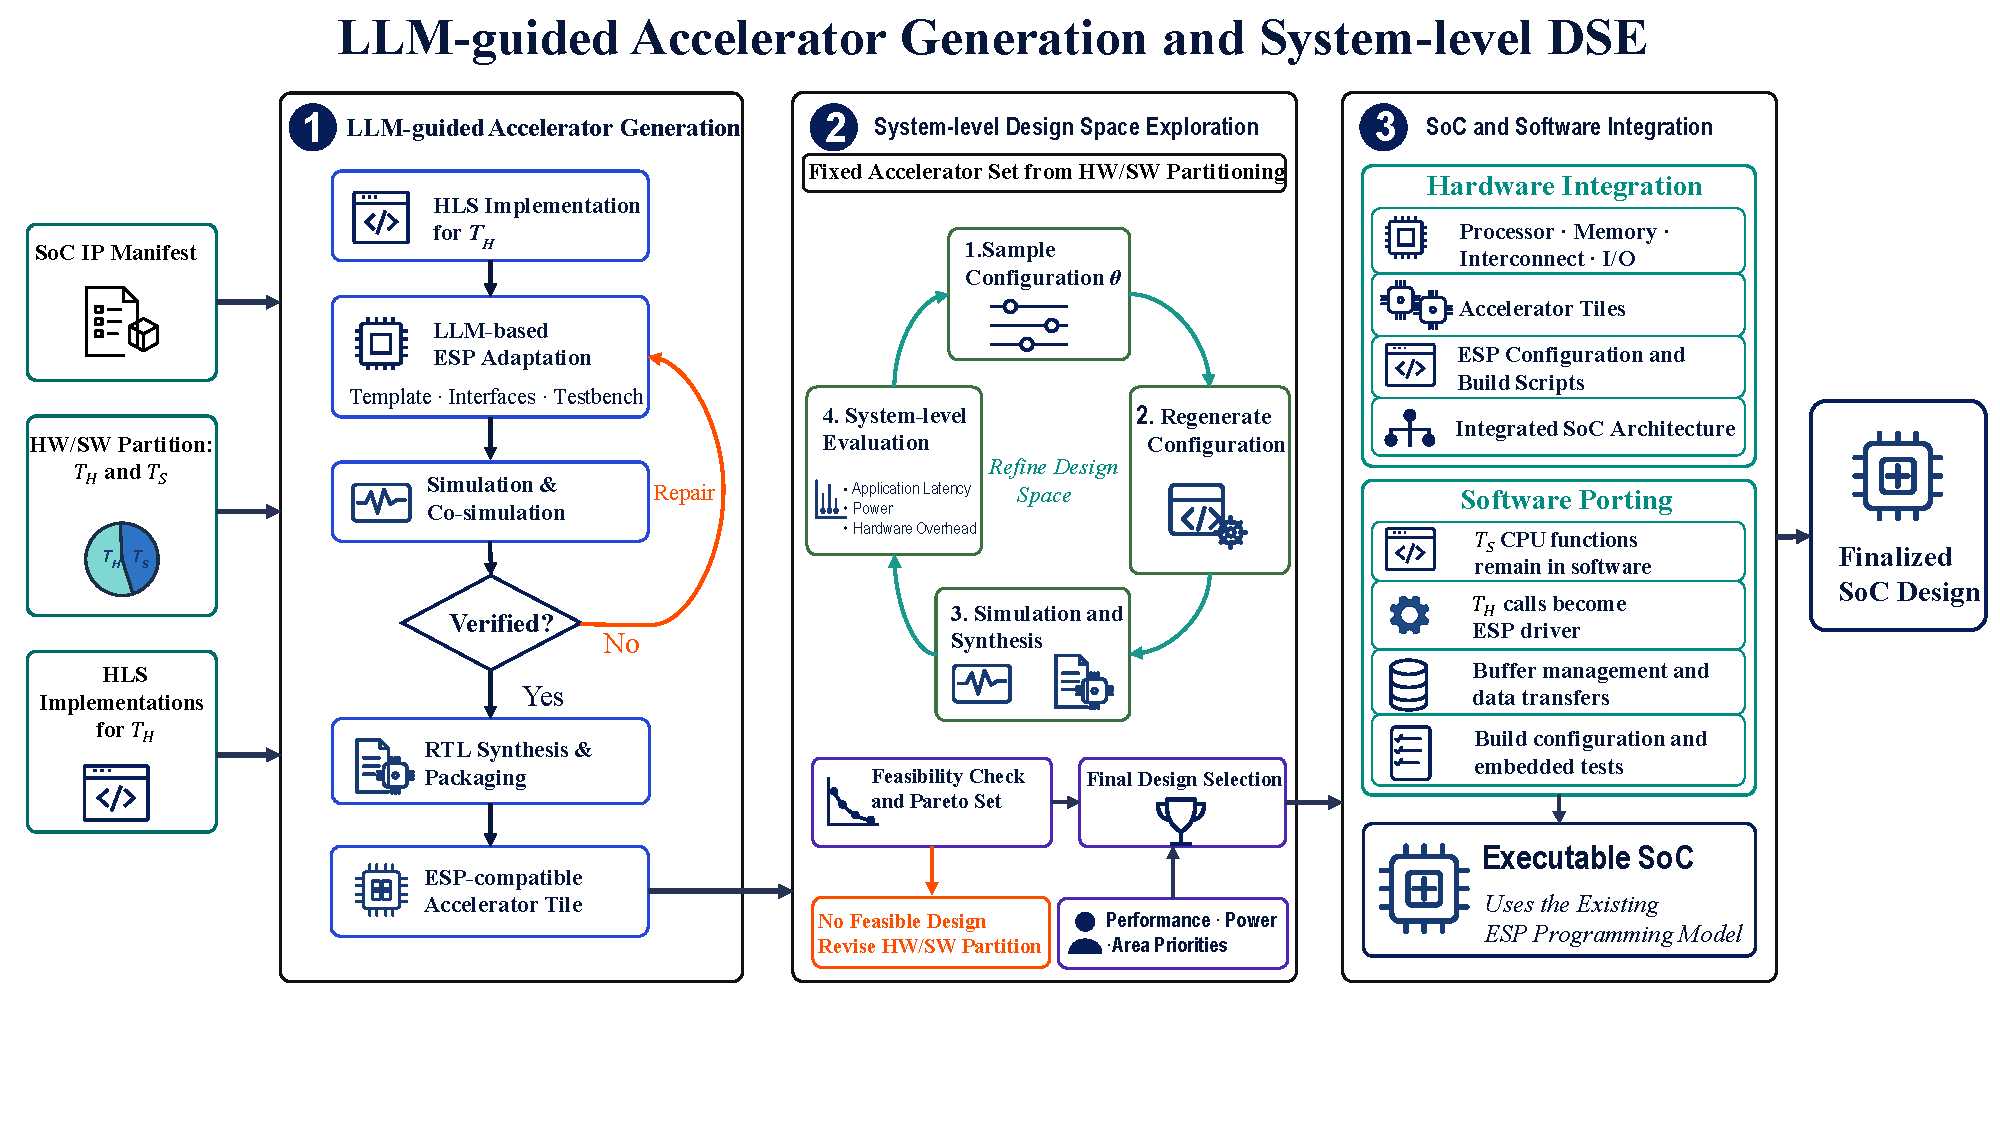
\includegraphics[width=0.92\textwidth]{pic/soc-generation.pdf}
    \caption{LLM-guided accelerator generation and system-level DSE. SoCPilot converts hardware-mapped functions into verified ESP-compatible accelerator tiles, integrates them with the selected system IPs and software, and refines the resulting SoC through system-level design space exploration. Infeasible designs trigger a revision of the hardware/software partition.}
    \label{fig:soc-generation}
\end{figure*} 


\textbf{Accelerator and SoC generation.}
SoCPilot automates the integration of HLS-generated accelerators into the ESP framework~\cite{7428012}. For each application function designated for hardware execution within $T_H$, the framework processes the synthesized hardware implementation and its interface metadata, encapsulating them into an ESP-compatible third-party accelerator. This encapsulation equips the module with the protocol adaptation, control, memory-access, and interrupt interfaces necessary for operation within the ESP architecture, while concurrently generating the requisite metadata for system-level composition. Subsequently, the packaged accelerator is registered with the ESP system-generation flow and instantiated as an accelerator tile based on the target SoC configuration. Prior to system integration, the accelerator undergoes comprehensive validation via C-level simulation, high-level synthesis, and C/RTL co-simulation, ensuring that only functionally verified hardware is incorporated into the final SoC.

Subsequently, SoCPilot constructs the target SoC by instantiating the chosen processor, memory subsystem, interconnect, I/O components, and accelerator tiles via the ESP system-configuration and generation flow. Based on the specified hardware-software partition, functions designated to $T_S$ remain processor-executed, whereas functions allocated to $T_H$ are mapped to the integrated accelerator tiles. SoCPilot generates the hardware integration scripts and build configurations required to synthesize the final SoC. The embedded application routines that configure, invoke, and communicate with the accelerators are manually implemented by the authors using ESP's established runtime API; they are neither generated nor modified by the LLM and are kept fixed during evaluation. Thus, the automated boundary of SoCPilot covers accelerator generation, packaging, SoC configuration, integration, and tool-flow orchestration, but not embedded application-code generation.

%%这需要确定dse是按照什么方式阐述
%目前是先dse生成soc之后没有进行dse
\textbf{System-level design space exploration.}
The initial partition reduces the search space by fixing which functions are implemented as accelerators. SoCPilot then explores a parameter vector $\boldsymbol{\theta}$ that covers the available processor configuration, cache hierarchy, interconnect settings, and candidate accelerator implementations produced by the HLS stage. Accelerator choices include pragma configurations and interface parameters; system choices include cache capacity and associativity, cache-line size, and NoC buffering. Table~\ref{table:node parameter-all} lists the principal dimensions used in the current implementation.
%%这个地方最终soc支持这么多但是在实际dse是仿真的dse并不支持这么多
\begin{table}[h]
     \vspace{-1em}
    \caption{Principal parameters for system-level DSE}
    \label{table:node parameter-all}
    \vspace{-0.5em}
    \resizebox{0.5\textwidth}{!}{
    \renewcommand\arraystretch{1.3}
        \begin{tabular}{cc}
        \hline
          \textbf{Design variable} & \textbf{Candidate values or source} \\ \hline
          Processor configuration & ESP-supported configurations \\
          Accelerator implementation & Pareto candidates from HLS \\
          HLS pragmas & Pipeline, unroll, and array partition \\
          Interface data width & ESP-compatible configurations \\
          Cache line size & 128, 256, 512 \\
          L2 sets & 32, 64 \\ 
          L2 ways & 2, 4, 8 \\
          LLC sets & 128, 256, 512 \\
          LLC ways & 4, 8, 16 \\
          NoC FIFO depth & 2, 4, 6 \\ \hline
        \end{tabular}} 
\end{table}

For every sampled configuration, SoCPilot regenerates the relevant ESP configuration and evaluates end-to-end latency together with the estimated area provided by the common area model. HyperMapper \cite{9124618} explores this latency--area design space: its surrogate model proposes new configurations, tool feedback updates the model, and points that violate the application-specific area constraint are discarded. The final design is selected from the feasible configurations according to the latency objective under the specified area budget. In contrast to hardware/software partitioning, this search performs fine-grained optimization around the current accelerator set. If no feasible design is found, SoCPilot returns to the previous stage and revises the hardware/software partition.

\subsection{FPGA Prototyping and Board Validation}\label{sec:soc-Prototyping}
The final stage converts the selected design point into an FPGA prototype. SoCPilot passes the finalized ESP configuration and packaged accelerator RTL to the existing ESP automation scripts \cite{10.1145/3466752.3480065}, which generate the FPGA project, perform synthesis and place-and-route, and produce the bitstream. The benchmark-specific embedded application and accelerator-control code is manually implemented using the ESP runtime API and compiled with the generated hardware image; it is not produced by the LLM.

The FPGA board is used to validate that the generated CPU--accelerator SoC boots, correctly invokes the selected accelerators, and produces application outputs consistent with the CPU reference. Board measurements provide end-to-end execution latency, including CPU execution, accelerator invocation, communication, and synchronization overhead. Area is evaluated separately using the analytical area model used by the partitioning and DSE stages; FPGA board validation is used for functional deployability and latency measurement rather than as the area metric.


% The success of LLMs across diverse domains motivates the development of SoCPilot, an LLM-driven framework for end-to-end SoC design automation. As illustrated in Figure~\ref{fig: overview}, SoCPilot takes natural language and high-level application descriptions as input and has four tightly integrated stages to generate optimized SoC designs automatically. Leveraging the LLM's strengths in natural language understanding, tool interaction, and code generation, the framework performs expert-level decision-making across the entire design flow including requirement analysis, hardware/software partitioning, design space exploration, and FPGA implementation. This end-to-end approach bridges the gap between abstract specifications and concrete hardware, significantly reducing manual effort while maintaining high design quality. In the following sections, we illustrate each stage of the SoCPilot pipeline in detail.

% \subsection{Design Requirement Interpretation}
% SoCPilot begins by leveraging LLMs to interpret natural language and high-level application descriptions, and to select appropriate Intellectual Property (IP) blocks from a pre-built library. However, user requirements can vary significantly, and there often exists a substantial semantic gap between these high-level specifications and the low-level abstraction of IPs available for integration. As a result, direct IP selection using LLMs tends to be unreliable and suffers from a low success rate due to ambiguity and misalignment.

% To address this challenge, we introduce an interpretation framework, illustrated in Figure~XXX. The core idea is to define an intermediate meta-representation—function specifications—that serves as a structured bridge between user requirements and available IP blocks. These specifications are derived from both user input and SoC design knowledge, capturing essential functional, performance, and interfacing attributes. Simultaneously, we construct a hierarchical IP library that categorizes components based on functionality, application domain, and hardware interface compatibility, making IP selection more structured and efficient. By leveraging both the function specifications and the organized IP library, the framework enables the LLM to perform iterative refinement: checking whether current selections satisfy user requirements and incrementally improving the design through guided revision.

% \begin{table*}[htb]
% \caption{Requirement-to-IP Taxonomy for SoC Customization}
% \centering
% \small
% \begin{tabularx}{\linewidth}{cllX}
% \toprule
% \textbf{Tier\footnotemark[1]} & \textbf{Category} & \textbf{Tag} & \textbf{Description / Examples} \\
% \midrule
% \multirow{1}{*}{T0} 
%   & Application Domain       & \texttt{domain} & AI inference, sensor hub, audio DSP, ISPs, etc. \\

% \midrule
% \multirow{4}{*}{T1}
%   & Compute                  & \texttt{cpu}, \texttt{dsp}, \texttt{ai} & RISC-V, Arm cores, DSPs, AI accelerators\\
%   & Memory and Cache         & \texttt{mem}     & DDR/LPDDR, SRAM, cache hierarchy and coherency, scratchpad \\
%   & Interconnect             & \texttt{noc}, \texttt{axi}, \texttt{pcie} & Mesh NoC, AXI buses, PCIe root complex \\
%   & I/O Interfaces           & \texttt{io}      & USB, SPI, I²C, CAN, MIPI CSI/DSI, GPIO \\

% \midrule
% \multirow{4}{*}{T2}
%   & Power and Energy         & \texttt{power}   & Power budget, DVFS, retention memory \\
%   & Security and Safety      & \texttt{sec}     & AES engine, secure boot, ASIL level \\
%   & Reliability / Lifetime   & \texttt{rel}     & ECC, watchdog, over-temperature protection \\
%   & Thermal and Packaging    & \texttt{pkg}     & Thermal budget, packaging constraints \\

% \midrule
% \multirow{1}{*}{T3}
%   & Integration Constraints  & \texttt{pkg}     & I/O count, physical interface compatibility (e.g., PHYs, pads) \\
% \bottomrule
% \end{tabularx}
% \label{tab:req_taxonomy}
% \end{table*}
% \footnotetext[1]{T0 anchors what the chip is for; T1 are primary hardware building blocks; T2 are cross‑cutting constraints; T3 are enablement and integration details.}

% \textbf{User Requirement Description:}
% The user input must comprehensively capture three key aspects: (1) high-level application intent, (2) design constraints (e.g., power, performance, area), and (3) input data types, as illustrated in Figure~\ref{fig:SoC requirements}. These descriptions provide the foundation for generating function specifications. To ensure accurate IP matching, the system must extract explicit functional requirements. For example, a communication IP should be described not only in terms of protocol but also in terms of throughput, latency, and real-time performance constraints. To obtain a complete and unambiguous specification, the framework engages in an interactive refinement process where the LLM incrementally prompts the user to clarify vague or missing parameters. This progressive dialogue ensures critical design constraints are fully captured before proceeding.

% \textbf{SoC Function Specifications:}
% Function specifications serve as an intermediate layer between human-centric requirement descriptions and machine-usable IP selection criteria. They abstract the system intent into a structured format consisting of (1) function descriptions (e.g., image processing, wireless transmission, signal processing), (2) function performance metrics (e.g., image processing throughput, latency, power), and (3) I/O interfaces (e.g., SPI, I2C). These specifications can be derived from prompt-engineered LLM queries and refined through external domain-specific rules or design heuristics. By converting user intent into formalized specifications, SoCPilot improves both the accuracy and interpretability of the IP selection process and supports reasoning across different layers of the SoC stack.

% \textbf{IP Library Construction:}
% The IP library is constructed as a hierarchical database of reusable hardware modules, indexed by functionality, performance, and interface compatibility. Each IP block is annotated with a descriptor that includes supported configurations, resource usage, verification status, and known integration dependencies. This structure enables rapid filtering and ranking of candidate IPs during the design process. The hierarchy supports inheritance of capabilities. For example, a generic DMA engine may have specialized variants for streaming video or memory-to-memory transfers. To further improve matching accuracy, the library supports semantic tags and metadata that can be directly queried or inferred by LLMs, enabling more context-aware recommendations.

% \subsection{Candidate Hotspot Extraction}
% Before constructing the task graph, SoCPilot first identifies a set of candidate hotspots within the input program. This screening is essential, as a full C application typically comprises initialization code, control-intensive routines, library wrappers, and error-handling paths—none of which are suitable accelerator targets. Moreover, reasoning across the entire program would inflate the LLM's context window and potentially bias task decomposition toward functions that are syntactically prominent but computationally insignificant. The hotspot extractor thus serves as a front-end filter that bridges the raw application and the subsequent LLM-guided decomposition stage.

% Our approach combines dynamic profiling and static code screening. At runtime, SoCPilot compiles and executes the target program under Callgrind to identify functions with high instruction-execution counts. The parser subsequently filters out system routines, library wrappers, loader symbols, and top-level entry points, retaining only application-defined functions that carry substantial execution cost. This yields a workload-specific view of acceleration potential, grounded in actual execution behavior rather than in source-code structure or function size alone.

% Dynamic cost alone is not sufficient, because an expensive routine may remain HLS-incompatible. SoCPilot therefore performs a lightweight static screening pass on each profiled function. The pass examines each function for regular loop structure, dynamic memory allocation, indirect memory access patterns, floating-point operations, and recursion, while also verifying that the function can be isolated with its required definitions and calling context. Regular loop-dominated functions are treated as direct candidates; important functions with HLS-unfriendly constructs are retained as refactoring candidates; high-risk functions remain software-mapped unless later design-space exploration (DSE) evidence motivates reconsideration.

% This three-tier classification establishes a principled candidate set for task-graph construction, balancing acceleration opportunity against HLS feasibility before LLM-based decomposition. SoCPilot subsequently constructs the task graph exclusively over this reduced program slice, rather than over the full application. The candidate set is both empirically derived from runtime profiles and constrained by HLS feasibility—this dual grounding gives the mapping and repair stages a principled basis for subsequent decisions.

% \subsection{Hardware/Software Partitioning} 
% Given the task graph extracted from hotspots, SoCPilot formulates the hardware/software mapping as a constrained selection problem rather than a full-program rewriting problem. The key insight is that, once hardware cost and performance benefit are both taken into account, the partitioning problem reduces to a knapsack-like optimization: each candidate task carries an acceleration benefit, a communication cost, and a resource footprint, while the system offers a finite hardware budget. Therefore, the objective is not to accelerate every eligible function, but to select a subset of tasks whose net benefit is positive and whose total resource consumption stays within system-level constraints.

% \textbf{Task and Communication Evaluation:} 
% To guide mapping decisions, SoCPilot conducts hybrid PPA profiling for each task and evaluates the communication overhead between dependent tasks:

% \begin{itemize}
%     \item \textbf{Hardware PPA Estimation:} Candidate accelerators are synthesized using Vivado/Vitis HLS. SoCPilot extracts latency, and resource utilization (DSP, LUT, FF, BRAM) from HLS synthesis reports. These metrics serve as early-stage PPA signals for mapping and DSE. 
    
%     \item \textbf{Software Runtime Estimation:} The execution time of CPU-mapped tasks is estimated using Sniper~\cite{sniper}, a parallel multicore simulator.
    
%     \item \textbf{Communication Model:} SoCPilot accounts for data movement by associating task-graph edges with data-transfer volume and platform-dependent transfer cost. When two dependent tasks are mapped to different execution domains, the mapping stage adds a communication penalty to the successor's earliest start time; when they remain in the same domain, this penalty is reduced or omitted  according to the platform policy. This lightweight penalty prevents the mapper from selecting accelerators whose compute benefit is offset by data-movement overhead.

% \end{itemize}

% \textbf{Partitioning algorithm.} 
% Based on the above estimates, SoCPilot formulates the initial mapping as a resource-constrained task-graph partitioning problem. Each candidate task is characterized by its estimated acceleration benefit, HLS-derived resource cost, and communication penalty incurred when data crosses the CPU/accelerator boundary. The current implementation addresses this problem using a greedy heuristic: candidates are ranked by their effective benefit under the resource budget, and a task is mapped to hardware only when its net benefit is positive and the cumulative resource usage remains within admissible limits. This stage does not pursue global optimality; rather, it yields a compact and interpretable initial hardware/software partition, which freezes the candidate accelerator set and provides the starting point for subsequent DSE over processor, cache, and HLS directive parameters.


% \begin{algorithm}
% \label{alg:hw-sw-partitioning}
% \caption{Greedy Hardware/Software Partitioning}
% \KwIn{Task set $T=\{t_1,t_2,\ldots,t_n\}$; resource budget $R_{\text{max}}$}
% \KwOut{Hardware task set $T_H$ and software task set $T_S$}


% $T_H \leftarrow \emptyset$, $R_{\text{used}} \leftarrow 0$\;


% \ForEach{task $t$ in $T$}{
%     $comm(t) \leftarrow \text{CommCost}(t)$\;
%     $(gain(t), resource(t)) \leftarrow \text{HardwareEstimate}(t)$\;
%     $value(t) \leftarrow gain(t) - comm(t)$\;
% }


% Sort $T$ in descending order by $value(t) / resource(t)$\;


% \ForEach{task $t$ in sorted $T$}{
%     \If{$value(t) > 0$ \textbf{and} $R_{\text{used}} + resource(t) \leq 
% R_{\text{max}}$}{
%         $T_H \leftarrow T_H \cup \{t\}$\;
%         $R_{\text{used}} \leftarrow R_{\text{used}} + resource(t)$\;
%     }
% }


% $T_S \leftarrow T \setminus T_H$\;
% \Return{$T_H$, $T_S$}
% \end{algorithm}


% Algorithm~\ref{alg:hw-sw-partitioning} summarizes the initial partitioning logic. Upon obtaining this partition, SoCPilot conducts DSE to refine the architectural and HLS directives around the selected hardware task set—covering processor configuration, cache hierarchy, loop pipelining and unrolling, array partitioning, and interface data-width policy. The finalized design point is then recorded as machine-readable evidence to support subsequent repair, packaging, and validation.

% \textbf{Architecture Optimization:}
% To refine the partition further, SoCPilot performs multi-objective architecture optimization across processor and accelerator configurations. To explore the parameter space, we apply Bayesian optimization via HyperMapper~\cite{9124618} to investigate trade-offs between power, performance, and area. The final design is selected from Pareto-optimal configurations that meet all design constraints.

% \subsection{SoC Generation and Parameter Finetuning}\label{sec:soc-generation}
% Following the hardware-software partitioning phase, our framework generates the corresponding HLS accelerator and the SoC on the ESP platform. Subsequently, the system performs RTL-level synthesis to obtain accurate PPA metrics, which drive a final optimization stage using Bayesian optimization, as illustrated in Figure \ref{fig:soc-generation}.

% The ESP platform\cite{7428012} serves as a heterogeneous integration framework that enables agile SoC development. Our framework leverages LLM capabilities to automate the ESP toolchain operation, effectively simulating a domain expert. Beginning with hardware-software partitioning results, the LLM first derives the accelerator's architectural parameters, including register configurations and interface specifications, to generate a parameterized ESP accelerator skeleton. During accelerator implementation, the LLM automatically applies ESP-compliant optimization techniques (double buffering) to the target code. 
% \lstset{
% 		language=C++, 
% 		linewidth=0.48\textwidth, 
% 		columns=flexible, 
% 		basicstyle=\ttfamily \fontsize{8pt}{9pt}\selectfont , 
% 		breaklines=true,
% 		frame=single, 
% 		keywordstyle=\textcolor{Orchid}, 
% 		commentstyle=\textcolor{Gray}, 
% 		stringstyle=\textcolor{Orange}, 
% 		emph={merge, merge_arrays, histogram, histogram_parallel, histogram_map, histogram_reduce, bfs_kernel, read_frontier_vertex, traverse, convolve, read_dataflow, compute_dataflow, empty, read}, 
%     	emphstyle=\textcolor{NavyBlue}
%     }
%     \begin{lstlisting}
% // source code: 
% void feedforward(int *input, int *weights, int *output, int input_size, int output_size) {
%     loop1: for (int i = 0; i < output_size; i++) {
%         int sum = 0;
%         loop2: for (int j = 0; j < input_size; j++) {
%             sum += input[j] * weights[i * input_size + j];
%         }
%         output[i] = activate(sum);
%     }
% }
% \end{lstlisting}
%  \begin{lstlisting}
% //Accelerator behavior implementation
% //use the double-buffer ESP-compliant code
% bool ping = true;
% bool out_ping = true;
% {
%     uint32_t in_length = INPUT_SIZE * OUTPUT_SIZE + INPUT_SIZE;
%     uint32_t out_length = OUTPUT_SIZE;
%     uint32_t input_index = 0;
%     uint32_t output_index = 0;
%     uint32_t sum = 0;
%     for (int in_rem = in_length; in_rem > 0; in_rem -= PLM_IN_WORD) {
%     //adding the directives from DSE results
%         HLS_UNROLL_LOOP(COMPLETE, 2);
%         uint32_t in_len = in_rem > PLM_IN_WORD ? PLM_IN_WORD : in_rem;
%         this->compute_load_handshake();
%         // Computing phase implementation
%         for (int i = 0; i < in_len; i++) {
%             HLS_UNROLL_LOOP(COMPLETE, 2);
%             uint32_t input_val;
%             uint32_t weight_val;
%             if (ping) {
%                 input_val = plm_in_ping[i % INPUT_SIZE];
%                 weight_val = plm_in_ping[INPUT_SIZE + (output_index * INPUT_SIZE) + (i % INPUT_SIZE)];
%             } else {
%                 input_val = plm_in_pong[i % INPUT_SIZE];
%                 weight_val = plm_in_pong[INPUT_SIZE + (output_index * INPUT_SIZE) + (i % INPUT_SIZE)];
%             }
%             sum += input_val * weight_val;
%             input_index++;
%             if (input_index % INPUT_SIZE == 0) {
%                 uint32_t activated = sum > 0 ? 1 : 0;
%                 if (out_ping) {
%                     plm_out_ping[output_index] = activated;
%                 } else {
%                     plm_out_pong[output_index] = activated;
%                 }
%                 sum = 0;
%                 output_index++;
%             }
%         }
%         ping = !ping;
%     }
%     this->compute_store_handshake();
%     out_ping = !out_ping;
%     {
%         this->process_done();
%     }
% }
% \end{lstlisting}
% For verification, the SoCPilot generates comprehensive testbenches by analyzing functional requirements. 
% \begin{lstlisting}
% //Testbench implementation for simulation
% // Initialize input 
% in = new int32_t[INPUT_SIZE * OUTPUT_SIZE + INPUT_SIZE];
% for (int i = 0; i < INPUT_SIZE * OUTPUT_SIZE + INPUT_SIZE; i++) {
%     in[i] = i % INPUT_SIZE;
% }
% // Compute golden output
% gold = new int32_t[OUTPUT_SIZE];
% for (int i = 0; i < OUTPUT_SIZE; i++) {
%     gold[i] = 0;
%     for (int j = 0; j < INPUT_SIZE; j++) {
%         gold[i] += in[j] * in[INPUT_SIZE + i * INPUT_SIZE + j];
%     }
%     gold[i] = gold[i] > 0 ? 1 : 0;
% }
% \end{lstlisting}

% All of these codes are integrated into corresponding code file and valid the right of accelerators using the toolchain of the ESP.
% SoCPilot automatically integrates all generated code modules into target files, verifies accelerator functionality through simulation, and generates rtl using Cadence Stratus HLS.
% When simulations fail, the LLM diagnostically analyzes error traces to iteratively refine both the implementation code and testbenches, automatically rebuilding the accelerator cosimulation. This closed-loop process effectively encapsulates domain expertise while maintaining full automation from specification to verified implementation.

% To enable comprehensive design space exploration and precise optimization, our framework performs system-level DSE based on post-synthesis simulation data. Given the constrained parameter space resulting from interdependent configurations (Table \ref{table:node parameter-all}), our framework employs post-synthesis PPA metrics as the primary evaluation criteria for DSE. We still perform multi-objective PPA optimization via Bayesian optimization (HyperMapper). If the optimization fails to converge within the prescribed iteration limit, the system automatically triggers hardware-software repartitioning to explore alternative design points, continuing this iterative refinement until a valid solution is obtained.


% \begin{figure}[htp]
%     \centering
%     \includegraphics[width=0.45\textwidth]{pic/SoC-generation.jpg}
%     \caption{Automatic Optimization Strategies Learning and Application}
%     \label{fig:soc-generation}
% \end{figure} 


% \begin{table}[h]
%      \vspace{-1em}
%     \caption{System-level design space exploration parameters}
%     \label{table:node parameter-all}
%     \vspace{-0.5em}
%     \resizebox{0.5\textwidth}{!}{
%     \renewcommand\arraystretch{1.3}
%         \begin{tabular}{cc}
%         \hline
%           \textbf{\begin{tabular}[c]{@{}c@{}}Architectural parameters \end{tabular}} &
%           \textbf{\begin{tabular}[c]{@{}c@{}}Candidate values \end{tabular}} \\ \hline
%            cache line size      &128, 256, 512              \\
%            L2 sets              & 32, 64                \\ 
%            L2 ways              & 2, 4, 8                \\
%            LLC sets             & 128, 256, 512                \\
%            LLC ways             & 4, 8, 16                \\
%            NOC fifo depth       & 2, 4, 6               \\        \hline
%         \end{tabular}} 
 
% \end{table}


% \subsection{FPGA Prototyping and ASIC Design }\label{sec:soc-Prototyping}
% Our framework implements a closed-loop verification and optimization pipeline that begins with automated FPGA prototyping. RTL designs are synthesized and implemented on target platforms while leveraging LLM-generated, ESP-compliant embedded verification code for comprehensive functional validation. During execution, the system continuously monitors runtime performance through ESP's API interfaces\cite{10.1145/3466752.3480065}, collecting critical metrics including accelerator execution times, interconnect communication latency, memory access patterns, and cache utilization statistics. The LLM re-optimizes SoC cache configurations (cache coherence modes, memory allocation policies, and NoC bandwidth allocation) based on actual workload characteristics.


% Current capabilities focus on functional validation and architectural optimization, with planned extensions to incorporate complete physical verification including design rule checking (DRC), layout versus schematic (LVS) verification, timing closure automation, and manufacturability analysis - ultimately bridging the gap between rapid prototyping and production-ready SoC implementation through this data-driven, closed-loop methodology.


